\documentclass[11pt,a4paper]{article}
\usepackage[a4paper,hmargin=1in,vmargin=1in]{geometry}
\usepackage{pgfplots}
\pgfplotsset{compat=1.17}

\usepackage[czech]{babel}
\usepackage[utf8]{inputenc}
\usepackage[T1]{fontenc}

\usepackage{stddoc}


\begin{document}

	\begin{titlepage}
        \begin{center}
            \vspace*{2cm}

            {\Huge Semestrální práce}\\[0.5cm]
            {\Large Analýza experimentálních dat}
            \vspace{2cm}

            
\includegraphics[width=0.9\textwidth]{src/logo_FEL.pdf}
            \vspace{2cm}

            \textbf{\LARGE Predikce úbytku mozkové hmoty z řeči a dalších klinických měření u roztroušené sklerózy}
            \vfill
            
            {\large Martin Šimák (\texttt{simakma5@fel.cvut.cz})}\\
            {\large Petr Šimek (\texttt{simekpe7@fel.cvut.cz})}\\
            {\large Jan Šmolcnop (\texttt{smolcjan@fel.cvut.cz})}
        \end{center}
    \end{titlepage}

	\newpage
	\section{Úvod}
            Tato práce se zabývá neurologickým onemocněním roztroušená skleróza (RS). Jedná se o závažnou nemoc postihující nervovou soustavu. \uv{RS je chronické zánětlivé onemocnění centrální nervové soustavy. Diagnóza vyžaduje průkazný nález zánětlivých ložisek, která jsou od sebe časově i prostorově oddělena, a vyloučení jiných zánětlivých, strukturálních, nebo dědičných stavů, které by mohly poukazovat na stejný klinický obraz.} \cite{nicholas2013} Diagnostika RS je problematická, jelikož se onemocnění projevuje v počátcích jen nepatrně. Celý proces odhalení nemoci se skládá ze 4 základních kroků. Nejprve odhalení ložisek, která nesmí mít jiné vysvětlení. Dále je třeba mít klinicky podložené příznaky, radiologická a laboratorní vyšetření. Nakonec je jedinec klasifikován, zda-li je RS pozitivní či negativní. Také může dojít k tomu, že splňuje jen některá kritéria a je nazván \uv{pravděpodobně pozitivním} \cite{mcdonald2001}.
            
            V dnešní době toto onemocnění postihuje asi 2,5 milionu lidí na světě a stojí miliardy dolarů ve veřejném zdravotnictví \cite{mcalpine2005}. Zatím nebyla nalezena žádná účinná léčba, ale probíhá mnoho studií, které se o to snaží. Zároveň je pro studium nemoci zapotřebí nalézt způsob predikce jejího vývoje, což je motivací této studie.
 
            Jedním z typických syndromů RS je úbytek mozkové hmoty viditelný na MRI skenu. Pro predikci úbytku mozkové hmoty bylo k dispozici 10 řečových parametrů: DDKR, DDKI, stdF0, Jitter, HNR DUS, RFA, IntSD, F0SD a NSR. Jejich definice a popis jsou v příloze v sekci \ref{sec:parametry}.
            
            \subsection{Otázky a hypotézy}
                Zprvu byly definovány otázky a k nim i hypotézy, dle kterých byly vybrány vhodné metody.

                \begin{enumerate}
                    \item \label{en:normalita}Jsou parametry z normálního rozdělení?
                        \begin{description}
                            \item[H0:] Zkoumaný parametr má normální rozdělení na zvolené hladině statistické\\ významnosti $\alpha = 0.05$.
                            \item[H1:] Zkoumaný parametr nemá normální rozdělení na zvolené hladině statistické \\významnosti $\alpha = 0.05$.
                        \end{description}
                    \item \label{en:korelace}Existuje nějaký vztah mezi mezi řečovými parametry? Existuje nějaký vztah mezi parametry mozkové hmoty?
                        \begin{description}
                            \item[H0:] Mezi parametry mozkové hmoty neexistuje korelace/lineární vztah, $\rho = 0$.
                            \item[H1:] Mezi parametry mozkové hmoty existuje korelace/lineární vztah, $\rho \neq 0$.
                        \end{description}
                    \item \label{en:vek}Má věk vliv na úbytek mozkové hmoty?
                        \begin{description}
                            \item[H0:] Úbytek daného typu mozkové hmoty v závislosti na EDSS, které popisuje míru postižení, nezávisí na věku.
                            \item[H1:] Úbytek daného typu mozkové hmoty v závislosti na EDSS, které popisuje míru postižení, závisí na věku.
                        \end{description}
                    \item \label{en:sex}Má pohlaví vliv na úbytek mozkové hmoty?
                        \begin{description}
                            \item[H0:] Úbytek daného typu mozkové hmoty v závislosti na EDSS, které popisuje míru postižení, je pro obě pohlaví stejný.
                            \item[H1:] Úbytek daného typu mozkové hmoty v závislosti na EDSS, které popisuje míru postižení, není pro obě pohlaví stejný.
                        \end{description}
                    \item \label{en:vhodne}Jsou všechny změřené řečové parametry vhodné pro popis nemoci? Není některý parametr stejný pro zdravé i nemocné?
                        \begin{description}
                            \item[H0:] Hodnoty daného parametru pro skupinu zdravých lidí a pro skupinu nemocných lidí vychází z rozdělení se stejnou střední hodnotou (resp. mediánem).
                            \item[H1:] Hodnoty daného parametru pro skupinu zdravých lidí a pro skupinu nemocných lidí nevychází z rozdělení se stejnou střední hodnotou (resp. mediánem).
                        \end{description}
                \end{enumerate}
        \subsubsection*{Dodatečné otázky}
            Dále jsme si položili následující otázky, které nelze považovat za statistické hypotézy, ale jsou významnými výstupy naší studie:
            \begin{enumerate}
                \item \label{en:rel} Které řečové parametry jsou relevantními ukazateli úbytku mozkové hmoty?
                \item \label{en:predikt}Lze ze zvolených parametrů spolehlivě predikovat úbytky mozkové hmoty?
                \item \label{en:vysledky}Dosahuje tento model lepších výsledků než jiné?
                \item \label{en:odhad}Lze odhadování úbytku mozkové hmoty nějakým způsobem zlepšit?
            \end{enumerate}
                
    \section{Metodika}
        \subsection{Popis dat}
            Cílem této práce bylo dle různých parametrů změřených z řeči predikovat úbytek mozkové hmoty u pacientů s RS. Celkem bylo změřeno 123 pacientů (MS) s klinicky diagnostikovanou RS, z toho 92 žen (75 \%) a 31 mužů (25 \%) (průměrný věk = 43,8 let, std = 10,8; průměrná délka trvání nemoci = 14,4 let, std = 7,6) a 60 zdravých kontrolních vzorků (HC). 23 pacientů (19 \%) bylo vážně postižených (EDSS $\geq5$), 65 (53 \%) mělo středně vážné příznaky (EDSS v intervalu $[2,5;5)$) a 35 (28 \%) mělo mírné příznaky (EDSS $<2.5$).

        \subsection{Použité metody}
            Jako první krok jsme zvolili provední metody LASSO za účelem zodpovězení otázky \ref{en:rel}. Díky tomuto kroku jsme hned ze začátku mohli vyloučit některé z naměřených parametrů, které nemají vliv na změnu mozkové hmoty. Dále jsme pomocí Shapirova-Wilkova testu vyšetřili normalitu zbylých parametrů (otázka \ref{en:normalita}) jakožto důležitý parametr pro použití dalších statistických testů. Další redukci dimenzionality úlohy poskytl test korelace (otázka \ref{en:korelace}). Následně jsme pomocí testu N-way ANOVA nalezli odpověď na otázky \ref{en:vek} a \ref{en:sex}. Pomocí T-testu, resp. Mannova-Whitneyova U-testu, jsme pro parametrické, resp. neparametrické, náhodné proměnné zjistili, zda je parametr pro subjekty zdravé a nemocné ze stejných rozdělení (otázka \ref{en:vhodne}). Na závěr jsme provedli fit lineárního regresního modelu, který slouží jako hlavní výstup studie a zároveň odpověď na otázky \ref{en:predikt}, \ref{en:vysledky} a \ref{en:odhad}.
	
	\section{Výsledky}
        \subsection{KDE a normalita dat}
            \begin{figure}[!ht] % NEDAT OBRÁZEK DO PŘÍLOH NA CELOU STRÁNKU????
                \centering
                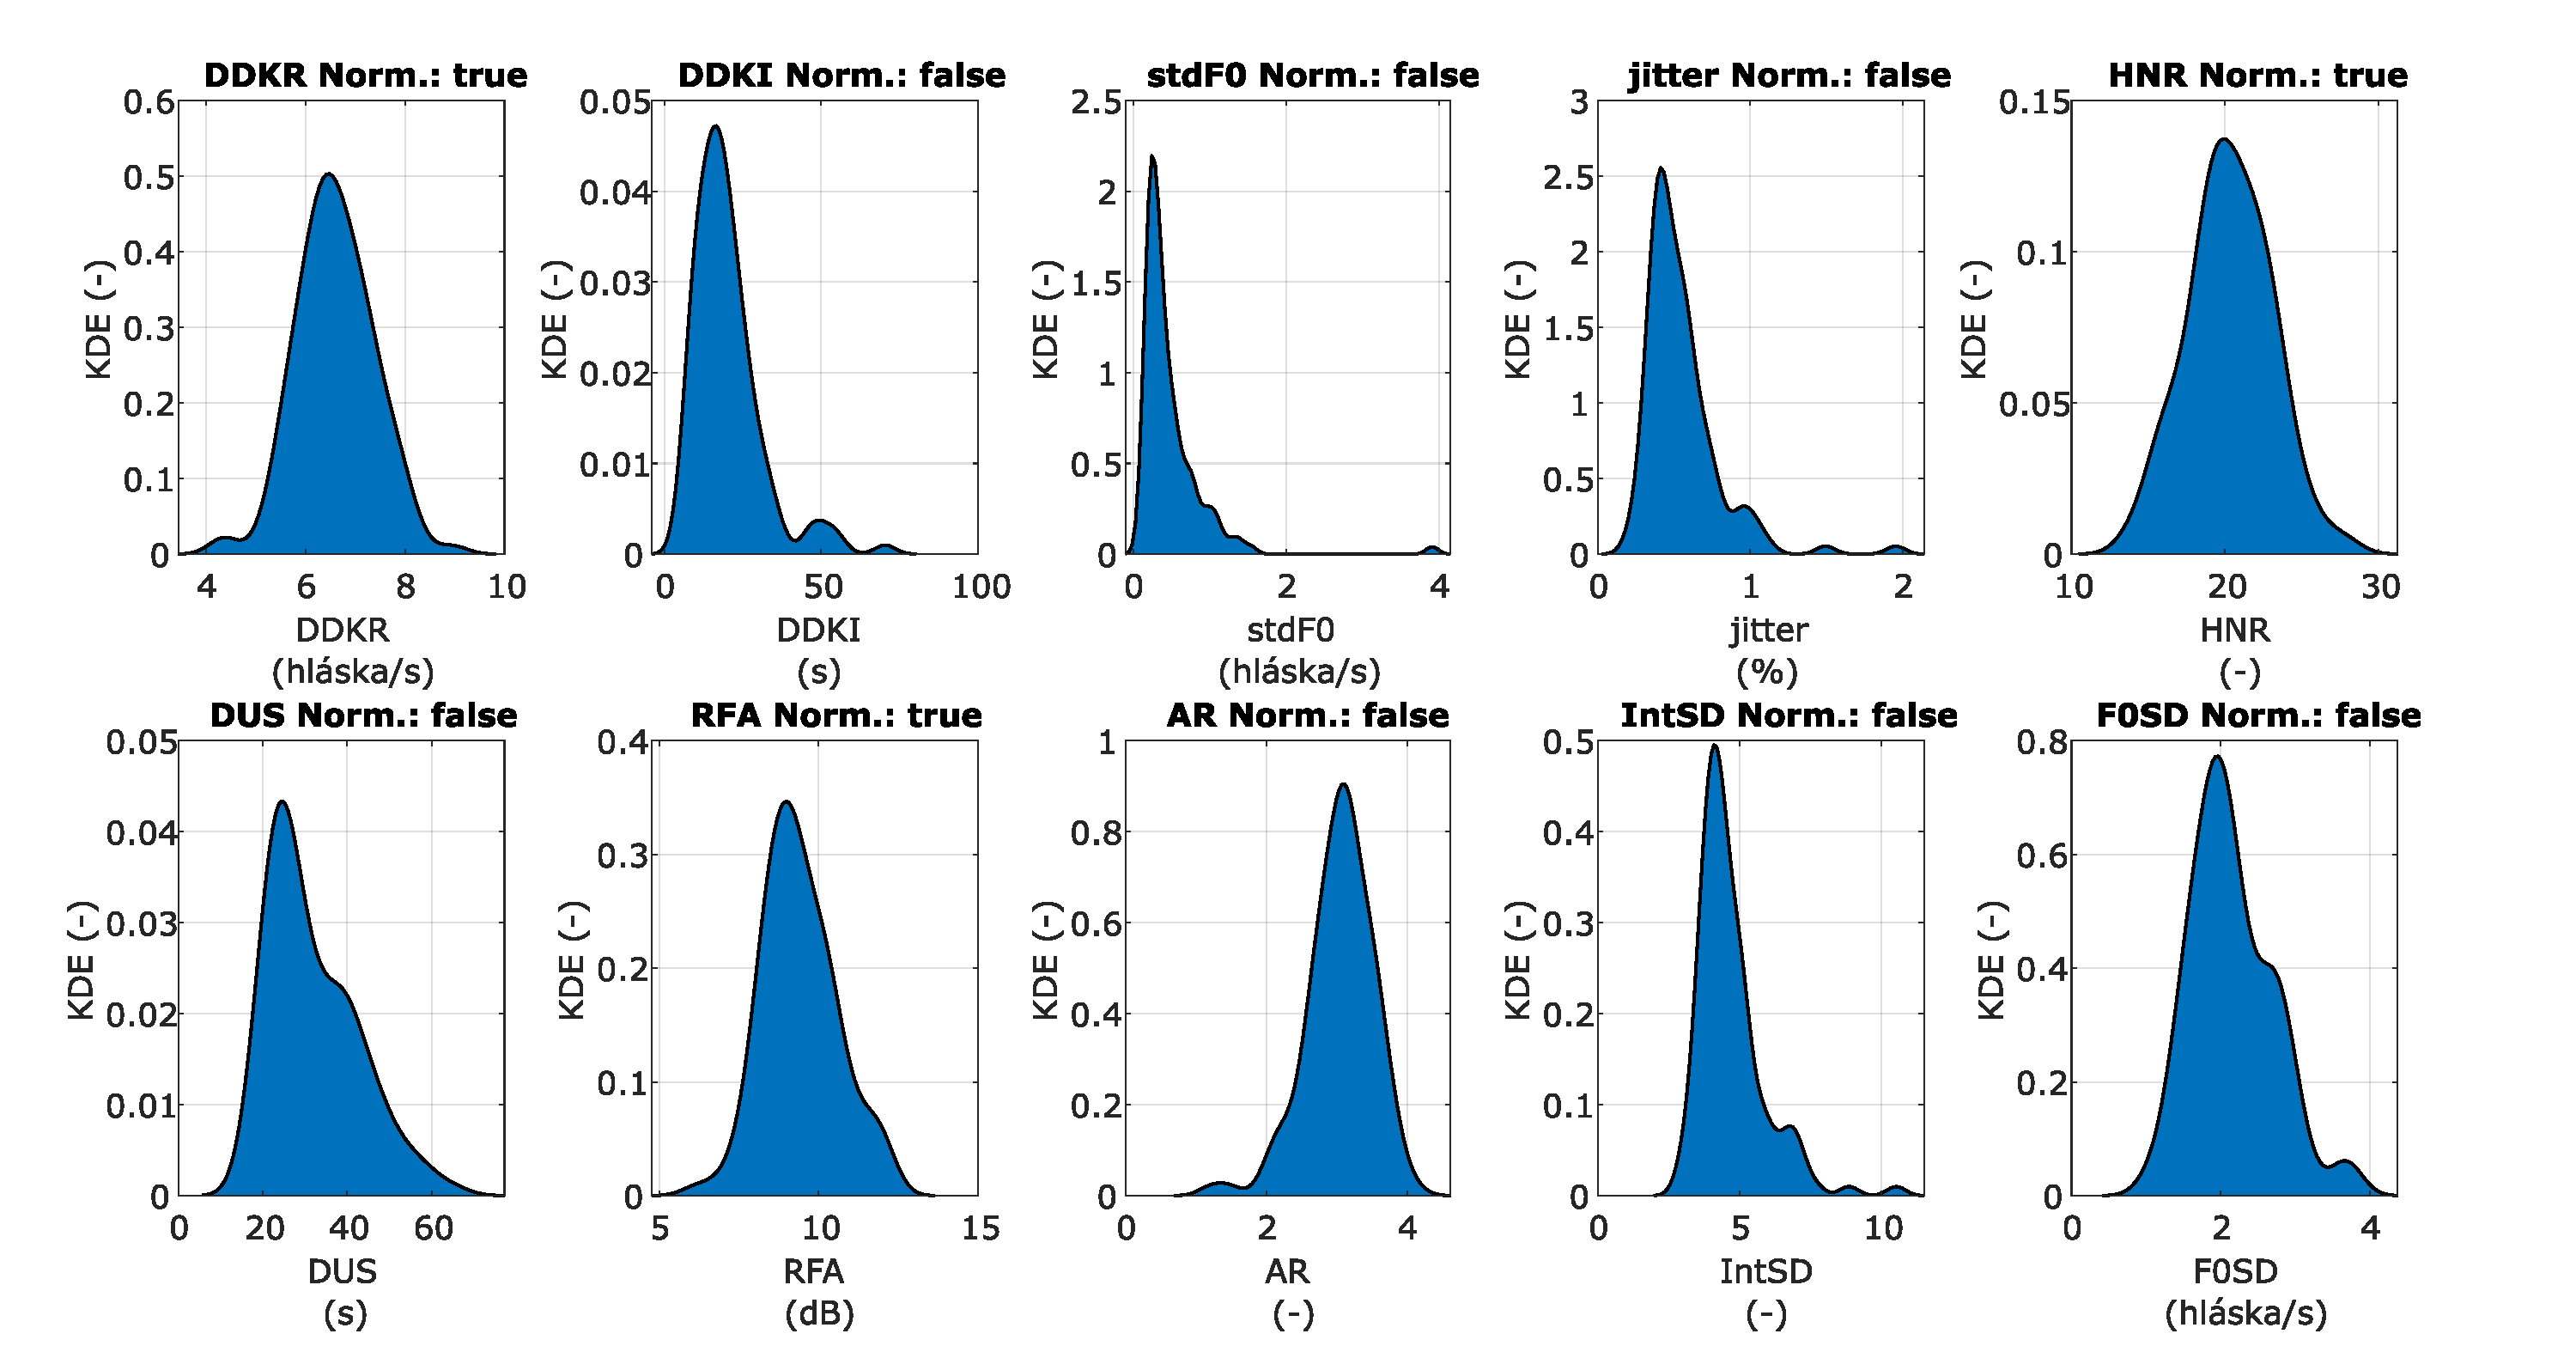
\includegraphics[width=\textwidth]{src/kde.pdf}
                \caption{Zobrazení KDE řečových parametrů. Zkratka Norm. znamená normalita. Hladina statistické významnosti $\alpha=0,05$.}
                \label{fig:kde}
            \end{figure}
            
        \subsection{LASSO}
            Na základě výsledků metody Lasso byly pro jednotlivé typy mozkových hmot určeny následující parametry jako relevantní:
            \begin{table}[!ht]
                \centering
                \begin{tabular}{c|c}
                    & Použité řečové parametry \\
                    \hline
                    White matter & StdF0, DUS, AR, IntSD \\
                    Gray matter & AR, IntSD \\
                    Cerebellar WM & DDKR, Jitter, HNR, AR \\
                    Cerebellar GM & DDKR, Jitter \\
                    Whole brain tissue & StdF0, Jitter, AR \\
                \end{tabular}
                \caption{Parametry, které byly použity pro model na základě metody Lasso.}
                \label{tab:lasso}
            \end{table}
         
        \subsection{N-way ANOVA pro věk a pohlaví}
            \begin{table}[hbtp]
                \centering
                \begin{tabular}{c|c|c|l}
                                   & Prob \textgreater F (Sex:EDSS) & Prob \textgreater F (Age:EDSS) &  \\ 
                                   \hline
                White matter       & 0,71          & 0,57  \\                     
                Gray matter        & 0,66          & 0,44  \\                 
                Cerebellar WM      & 0,17         & 0,63     \\                  
                Cerebellar GM      & 0,48          & 0,36      \\           
                Whole brain tissue & 0,65           & 0,72       \\                  
                \end{tabular}
                \caption{Výsledky N-way ANOVA pro pohlaví a věk}
                \label{tab:anovy}
            \end{table}
            
            
        \subsection{T-test/Mann-Whitney U-test}
            Na základě provedeného Mann-Whitney U-testu pro parametr IntSD vychází, že pro obě skupiny dat, tedy zdraví (med = 4.53) a nemocní (med = 4.34), pochází parametr IntSD z~rozdělení se stejným mediánem (z = -0.24, p-value = 0.81), tedy není ovlivněn tím, jestli je daný člověk nemocný.

            Pro všechny ostatní řečové parametry vychází, že pro zdravé i nemocné vychází daný parametr z rozdělení s různými středními hodnotami (resp. mediány).
        
        \subsection{Lineární regresní model}
            \begin{table}[!ht]
                \centering
                \begin{tabular}{c|c c|c c|c c}
                    & R-adj. (\%) & RMSE & R-adj. (\%) & RMSE& R-adj. (\%) & RMSE \\
                    \hline
                    White matter & 24 & 2,33& 24,9 & 2,32& 27,2 & 2,28\\
                    Gray matter & 16,7 & 2,27& 17,4 & 2,27& 17,5 & 2,27\\
                    Cerebellar WM & 13 & 0,28& 20,8 & 0,26& 24,9 & 0,25\\
                    Cerebellar GM & 12,1 & 0,72& 20,6 & 0,65& 23,9 & 0,64\\
                    Whole brain tissue & 23,2 & 4,27& 34,9 & 3,83& 34,6 & 3,87\\
                \end{tabular}
                \caption{Kvalitativní parametr lineárního regresního modelu. První sloupec: model naší studie, použity řečové parametry. Druhý sloupec: použity jen klinické parametry. Třetí sloupec: použity řečové i klinické parametry.}
                \label{tab:fitlm}
            \end{table}
        
    \section{Diskuse}
        Práce s parametry, kterou jsme provedli v rámci studie jako první krok, se ukázala jako velmi výhodná. V tomto ohledu jsme nejprve provedli T-test, resp. Mannův-Whitneyův U-test, pro potvrzení efektu onemocnění RS na výsledky řečových parametrů, na základě čehož jsme byli schopni označit hned jeden řečový parametr za nerozhodující. Následně pomocí zkoumání interakcí pohlaví-onemocnění a věk-onemocnění, přičemž pro hodnocení závažnosti onemocnění jsme v rámci tohoto testu používali parametr EDSS, pomocí metody N-way ANOVA jsme potvrdili, že závažnost onemocnění není závislé na věku ani na pohlaví, tj. že není zapotřebí rozdělovat data do věkových/pohlavních skupin a počítat regresní modely pro tyto skupiny zvlášť. Na závěr analýzy zpracovávaných parametrů jsme pomocí LASSO \emph{feature selection} metody dokázali vyloučit hned několik dalších parametrů, které na predikci úbytku mozkové hmoty nemají vliv.

        Výsledky výše zmíněné analýzy jsme použili pro sestavení lineárních regresních modelů pro predikci úbytku mozkové hmoty (pro každý parametr zvlášť). Výsledné modely jsou schopné predikovat úbytek mozkové hmoty srovnatelně přesně jako parametry MSFC aktuálně používané pro diagnostiku onemocnění RS.
        
        Za přínos studie lze považovat fakt, že kombinací námi zvolených řečových parametrů a stávajících parametrů MSFC lze sestrojit lineární regresní model dosahující lepších parametrů přesnosti predikce než doposud.

        Za nedostatek/limitaci studie lze naopak považovat mírně nekorektní přístup během analýzy pomocí metody N-way ANOVA, kterou jsme použili i na parametry, jejichž test normality vyšel negativně. Metodu jsme se ale i přesto rozhodli použít, neboť jejich \uv{míru neparametričnosti} jsme posoudili jako nízkou.

    \section{Závěr}
        Výsledky počáteční analýzy parametrů poskytují zhodnocení artefaktů řeči jako biomarkerů úbytku mozkové hmoty. Tento výběr lze považovat za hodnotný výstup práce.
        
        Hlavním výstupem práce jsou predikční modely postavené právě na výše zmíněných parametrech. Kvalitativní parametry těchto modelů nejsou sice příliš přesvědčivé ($R_\mathrm{adj} \approx 0.2$), nicméně lineární regresní modely postavené na stávajících metrikách MSFC dosahují srovnatelné přesnosti. Navíc kombinací všech zmíněných parametrů jsme schopni dosahovat mírně vyšší přesnosti modelu než pouze za pomoci parametrů MSFC.
\newpage

    \section{Přílohy}
        \subsection{Popis parametrů} \label{sec:parametry}
            \begin{enumerate}
                \item DDKR - Odhaduje se jako inverze mediánu trvání dvou po sobě jdoucími nástupy hlasu. Abnormálně pomalá rychlost pohybu artikulátorů.
                \item DDKI -  Odhaduje se jako směrodatná odchylka naměřených dob trvání mezi po sobě následujícími nástupy hlasu. Nepravidelné nebo časově omezené opakované pohyby.
                \item stdF0 - Počítá se jako směrodatná odchylka zjištěného modálního F0 v půltónech odhadnutá pomocí mediánu absolutní odchylky. Nepravidelné nebo časově omezené vibrace hlasivek.
                \item Jitter -  Frekvenční poruchy. Drsný a chraplavý hlas.
                \item HNR - Množství šumu ve znělé řeči. Drsný a chraplavý hlas.
                \item DUS - Medián neznělých stopových souhlásek určený z bimodálního rozložení délky neznělých stopových souhlásek a neznělých frikativ pomocí algoritmu maximalizace očekávání.Perioda stopových souhlásek je prodloužena třetím šumem nedostatečně uzavřených artikulátorů.
                \item RFA - Útlum rezonanční frekvence, definovaný jako rozdíly mezi maximy druhé formantové oblasti a minimy lokální oblasti antiformant. Hypokineze vede k poklesu spektrální energie v důsledku útlumu artikulačních pohybů.
                \item IntSD - Směrodatná odchylka obrysu intenzity řeči extrahovaného z hlásek. Hypokineze vede ke snížení amplitudy dýchacích a tyrearteonidálních svalů.
                \item F0SD - Směrodatná odchylka obrysu základní frekvence převedená na půltónovou stupnici. Hypoteneze způsobuje sníženou amplitudu pohybu hlasivek, což vede ke glotální inkopetenci.
                \item NSR -  Celkový počet slabik vydělen celkovou délkou řeči. Pomalost jednotlivých pohybů artikulátorů.
            \end{enumerate}
\newpage
\bibliographystyle{plain}
\bibliography{refs}

\end{document}